\chapter{Methods, approach and materials}
\label{chap:methods}


\section{Interview}
\label{sec:interview}
Interviews are an essential part for each research. In order to gain a deeper understanding and a good overview regarding ASD test and screening methods for autism, interviews with medical - and child care personnel were planned. Additionally, information about the assessment of motor coordination skills used in Norway and Germany were of great importance.
Surprisingly, it was quite challenging to find people who have some kind of experience in the field of ASD. It seemed that only specialist in psychology could provide professional and deeper background information. For that reason, the interviews in this study were only in form of a brief conversation. However, the information gained during those conversations was useful and enlightening.


\subsection{Summary and conclusion of the interviews}

The interviewees provided insights in how Autism is handled in school environment and in context with ergo-therapy.  

The conversations revealed that children usually are not tested for Autism in preschool, however in case of observed abnormalities they will talk to the parents and recommend a further investigation with a psychologist specialized in child behaviour and development. Abnormal behaviour of children is characterized by language delay, dislike of body contact, dislike of noise and difficulties in understanding face mimic.
Additionally, the conversation also revealed that screening routines for children that could discover deficit as for instance autism is in general not carried out due to the poor time capacity and cost.
On the other hand, an ergo-therapist explained that it is hard to detect autism by testing fine-motor performance. However, children with autism would have problems to understand a certain task or game rules. Furthermore, receptive behaviour is also an distinguish sign for autism.
She also mentioned the problem with poor empathy and recognition of facial expression.

To conclude, evaluation of children's motor performance may not be a sufficient approach in order to discover Autism. Many other factors need to be considered when dealing with this problem. 



\section{Game design, prototype and limitation}
\label{sec:prototype}


\subsection{Leap Motion Device}

The Leap Motion device was purchased second hand on Finn. \footnote{www.finn.no} The V2 desktop tracking installation files which included the SDK version v2.3.1 were downloaded from Leap Motion website. \footnote{ www.leapmotion.com} The installation was straightforward and the device could immediately be connected to the PC and used with the Leap Motion visualizer.

\begin{figure}[h]  %t top, b bottom, p page | you can also use h to try to get the figure to appear at the current location
  \centering
  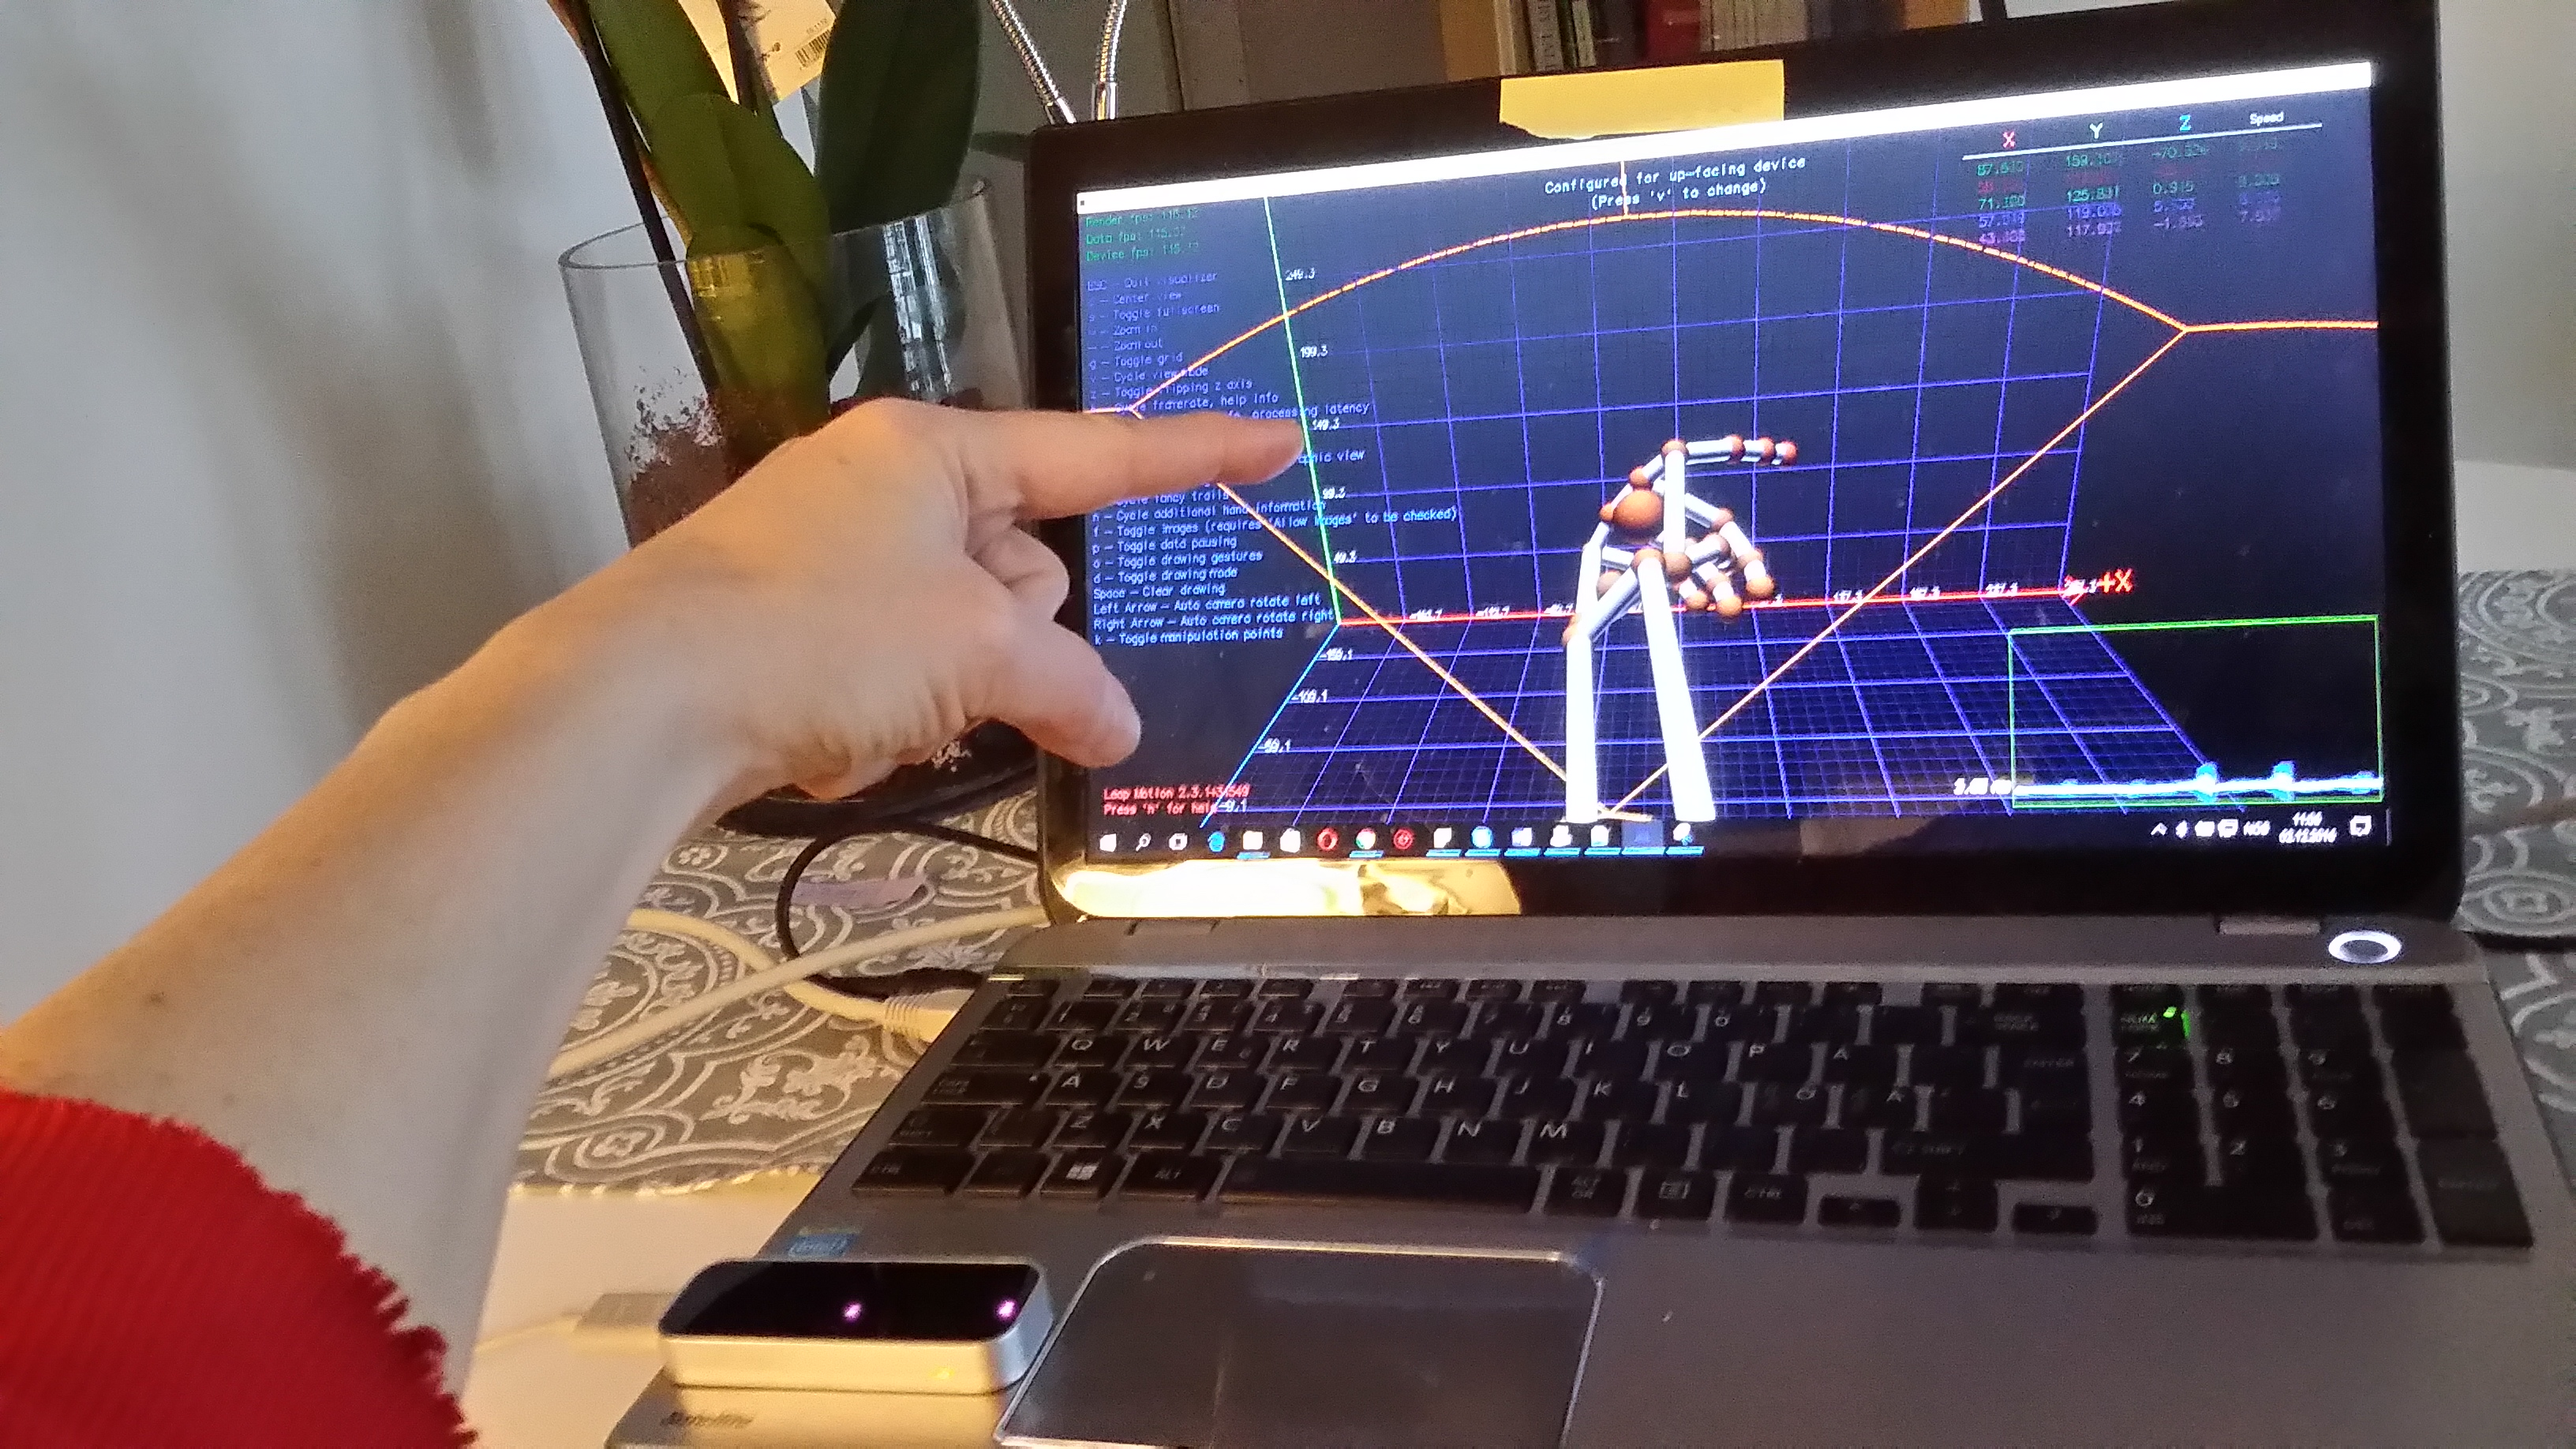
\includegraphics[width=.5\textwidth]{figures/LMvisualizer.jpg}
  \caption[Leap Motion visualizer.]{Leap Motion visualizer.}
  \label{fig:setup}
\end{figure}

The Java SDK documentation provided a good overview of the tracking data, hardware and software and showed how to get started with the Leap Motion API which was an excellent help during the whole prototyping process.

\subsection{Choosing a prototype tool}

A software prototype for test purpose was necessary to develop for this project. In order to accomplish the task it was essential to find a tool that could be used to create a simple and fast prototype and additionally is compatible with the Leap motion sensor. A quick Google search suggested Processing \footnote{https://processing.org/} which is a free open-source software. According to processing.org, the software is built particular within visual arts but also used for animation, installation products and interactive experience. It is a convenient prototype tool because it contains a integrated graphical user interface and additionally it is possible to use Java programming language in a simplified form.
Processing could also be used as a bridge between Leap Motion and Eclipse \footnote{https://eclipse.org/} which is known as an essential tool for Java developer.  Nevertheless, using Eclipse would be extensive and the setup would be more time consuming even if this would have been a more professional approach.

However, for this project, a simple and fast prototype was completely sufficient. For that reason, Processing was a suitable option. For the prototype development, Processing version 3.3.6 was installed locally.


\subsection{Game design}

In the initial design stage the idea of the whole system was sketched. In this stage the system had five modules. However, only one module could be implemented for this project due to the time limit.

\begin{figure}[h]  %t top, b bottom, p page | you can also use h to try to get the figure to appear at the current location
  \centering
  \includegraphics[width=.6\textwidth]{figures/sketch_wholeSystem.jpg}
  \caption[Idea generating.]{ Idea generating for the whole system}
  \label{fig:setup}
\end{figure}

For this project, the module "Mole in the hole" was chosen to implement further.

\begin{figure}[!h]  %t top, b bottom, p page | you can also use h to try to get the figure to appear at the current location
  \centering
  \includegraphics[width=.6\textwidth]{figures/prototypeSketch.jpg}
  \caption[Sketch Mole in the hole.]{Sketch: Mole in the hole}
  \label{fig:setup}
\end{figure}

At the second stage of the design process the background picture and figures needed to be created.The background picture was created in Adobe illustrator, version CS4. A photo illustrating the forest floor was downloaded free from Pixaby \footnote{www.pixaby.com} and used for the upper part of the game’s canvas. The underground was drawn as a vector art to make it more childlike. 
A grid was drawn and used as dimension and measurement aid for the white path. This was needed to simplify the programming implementation that used the same grid size. However, the grid was just an drawing aid and was not visible in the end product.

\begin{figure}[h]  %t top, b bottom, p page | you can also use h to try to get the figure to appear at the current location
  \centering
  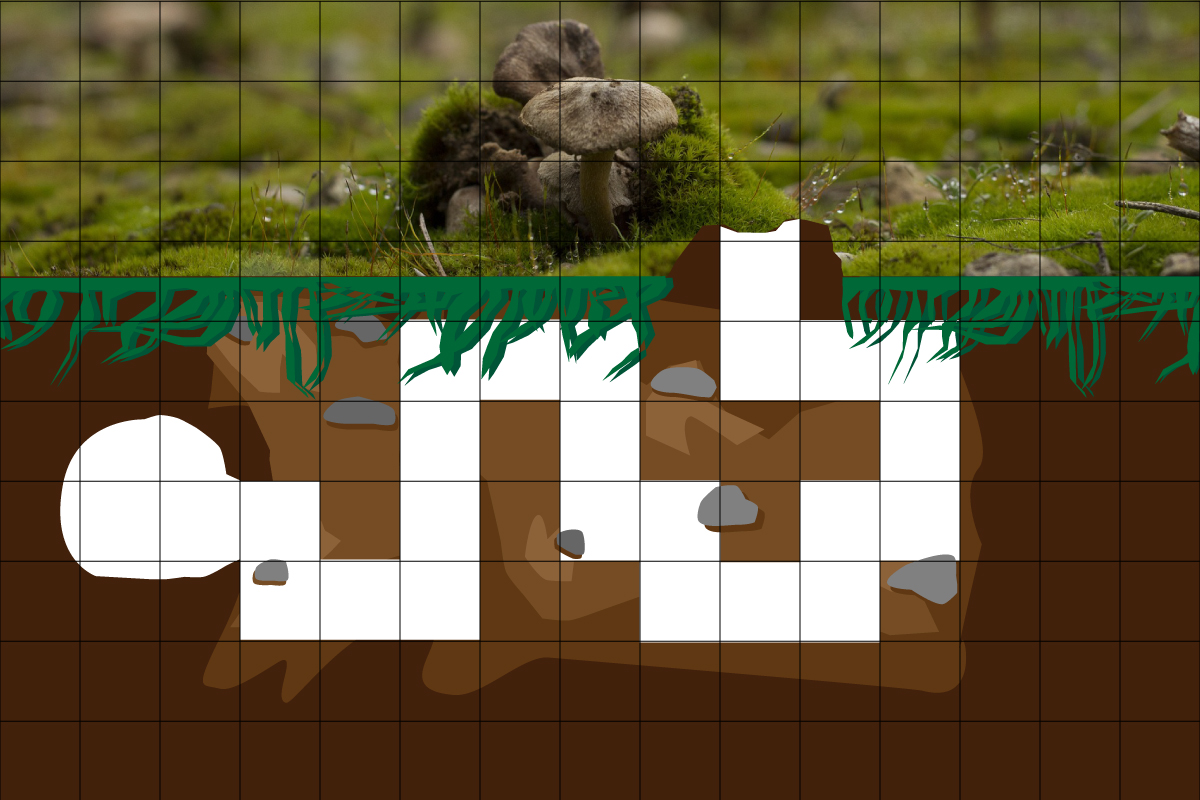
\includegraphics[width=.5\textwidth]{figures/Mole-in-the-hole-800x1200-GRID.jpg}
  \caption[Mole in the hole grid.]{Mole in the hole - grid.}
  \label{fig:setup}
\end{figure}

The five mole states and the stopwatch were drawn as a vector graphic in Adobe Illustrator, as well.

\begin{figure}[h]  %t top, b bottom, p page | you can also use h to try to get the figure to appear at the current location
  \centering
  
\includegraphics[width=.1\textwidth]{figures/MoleWait.png}
   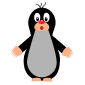
\includegraphics[width=.1\textwidth]{figures/MoleAttention.png}
   
\includegraphics[width=.1\textwidth]{figures/MoleJump.png}
   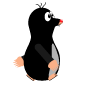
\includegraphics[width=.1\textwidth]{figures/MoleGo.png}
   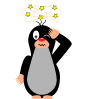
\includegraphics[width=.1\textwidth]{figures/MoleKaBoom.png}
  \caption[Mole's states.]{ The Mole's states: wait, attention, ready, go, hit.}
  \label{fig:setup}
\end{figure}

\begin{figure}[h]
  \centering
  
\includegraphics[width=.1\textwidth]{figures/timer.png}
  \caption[Timer]{Timer}
\end{figure}


The third design stage focused on illustrating the implementation and demonstrated the solution to the given problem.
A flow diagram was created for a better understanding of the design process and to analyze design problems. It illustrates the process stages and the conditions during the process from start point to the end point. 

\break

\begin{figure}[h]
    \centering
    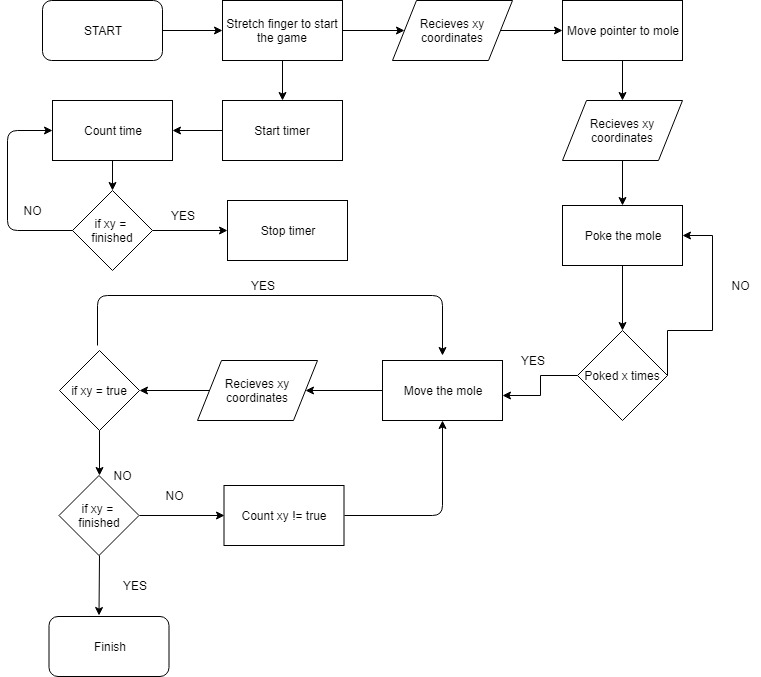
\includegraphics[width=.8\textwidth]{figures/FlowDiagram.jpg}
    \caption[Flow diagram: game design]{Flow diagram illustrates the game process}
    \label{fig: flowdiagram}
\end{figure}


\subsection{Prototype implementation}

In Processing, in order to make an animation or a interactive program, a predefined structure is used which includes a setup() and a draw() function. The setup() function runs only ones at the start whereas the draw() function loops continuously until the program is terminated or the noLoop() command appears in the code.
In the setup() function, the initial environment property as for instance the size of the canvas is defined  (size()).  In the draw() function, code that is meant to run continuously is defined here, like for instance the background() property. 

The framework would look likes this:
\lstset{frameround=tttt}
\lstset{frame=single}
\lstset{xleftmargin=.05\textwidth, xrightmargin=.05\textwidth}
\lstset{language=Java}
\begin{lstlisting}[caption = {Processing framework}, label={lst:Java}]
        void setup(
        {
            size();
        }
        void draw()
        {
            background();
        }

\end{lstlisting}

The program code for the module “Mole in the hole” implemented functions from the Leap Motion API. In order to use these functions the leap Motion library needed to be imported.

\lstset{language=Java}
\begin{lstlisting}[caption = {Leap Motion library}, label={lst:Java}]
import com.leapmotion.leap.*;
\end{lstlisting}

To connect to the Leap motion device a controller object was created

\lstset{language=Java}
\begin{lstlisting}[caption = {The code for touch zone}, label={lst:Java}]
Controller leap;
\end{lstlisting}

In setup() the controller was initialized as followed in order to establish a connection.

\lstset{language=Java}
\begin{lstlisting}[caption = {The code for touch zone}, label={lst:Java}]
leap = new Controller();
\end{lstlisting}

In order to make it easier to map position in the Leap Motion coordinate system an interaction box was initialized. The position within the 2D coordinate system was defined as X, Y which are coordinates for the hand and finger position. 

\lstset{language=Java}
\lstset{breaklines=true,postbreak=\mbox{{\color{blue}\tiny$\rightarrow$}}}
\begin{lstlisting}[caption = {The code for touch zone}, label={lst:Java}]

InteractionBox iBox = leap.frame().interactionBox();
Pointable pointable = leap.frame().pointables().frontmost();
Vector normalizedPosition = iBox.normalizePoint(pointable.stabilizedTipPosition());
float pixelX = normalizedPosition.getX() * windowWidth;
float pixelY = windowHeight - normalizedPosition.getY() * windowHeight;
int cx = (int) pixelX - 10;
int cy = (int) pixelY - 100;

\end{lstlisting}

Finger are recognize by the pointable class. The pointable.Zone defines the state of the current pointable object.

\lstset{language=Java}
\begin{lstlisting}[caption = {The code for touch zone}, label={lst:Java}]
 Pointable.Zone fingerzone = pointable.touchZone();
\end{lstlisting}

The touch zone is defined by three states:(see Leap Motion API reference for more information)
\begin{enumerate}
    \item ZONE\_NONE (pointable distant from the touch panel)
    \item ZONE\_HOVERING (is near the touch plane)
    \item ZONE\_TOUCHING (penetrates the touch plane)
\end{enumerate}




\lstset{language=Java}
\begin{lstlisting}[caption = {The code for touch zone}, label={lst:Java}]

            switch (pointable.touchZone()){
            case ZONE_NONE:
              //Handle distant pointable
              image(MoleState1, 80, 480);
              break;
            case ZONE_HOVERING:
              //Handle pointable near touch plane
              hide(MoleState1);
              image(MoleState2, 80, 480);
              break;
            case ZONE_TOUCHING:
              //Handle pointable penetrating touch plane
              counterTouching = counterTouching + 1;
              image(MoleJump, 80, 480); 
              break;
            default:
              //Handle error cases...
              break;
            }//end switch
          
\end{lstlisting}

A new finger object is created and initialized that starts the timer:

\lstset{language=Java}
\begin{lstlisting}[caption = {The code for touch zone}, label={lst:Java}]
  Finger finger = new Finger(pointable);
  if(finger.isExtended())
  {
    Timer(1);
  }
\end{lstlisting}

\break
%\break
In this game an invisible grid was drawn over the whole canvas size. Each grid cell had a size of 80 x 80 px. The mole’s hole and the way out was marked with white cells which x-y coordinates were stored as true-value in a two dimensional array.

\begin{figure}[h]  %t top, b bottom, p page | you can also use h to try to get the figure to appear at the current location
  \centering
  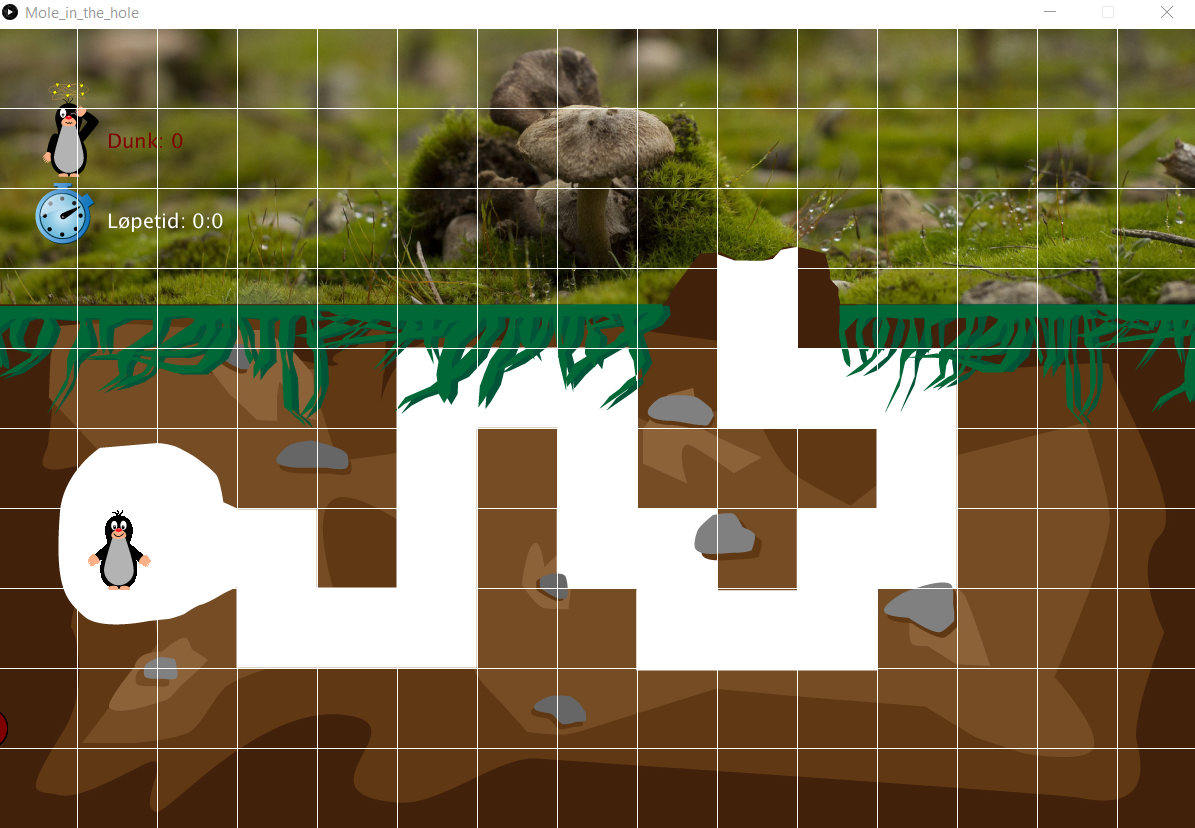
\includegraphics[width=.5\textwidth]{figures/Grid-processing-Mole_in_the_hole.png}
  \caption[Mole in the hole grid processing.]{Mole in the hole. Grid is drawn with a for loop.}
  \label{fig:setup}
\end{figure}

The pointer is activated by stretching the finger and pointing forward. The point moves in relation to the finger’s x,y coordinate. When the pointer hovers the mole, the mole changes state from “wait” to “attention”. When the Hole is poked his state will change from “attention” to “ready”. It needs about two til three pokes until the mole state changes to “go”. From that point the pointer disappear and only the mole moves and follows the finger’s position. All moves that are defined as false are counted as “hit”. The games is finished when the mole reaches the exit. The game counts the amount of hits and the elapsed time. The timer starts when the finger is stretched and the participant is ready to go.

\begin{figure}[h]  %t top, b bottom, p page | you can also use h to try to get the figure to appear at the current location
  \centering
  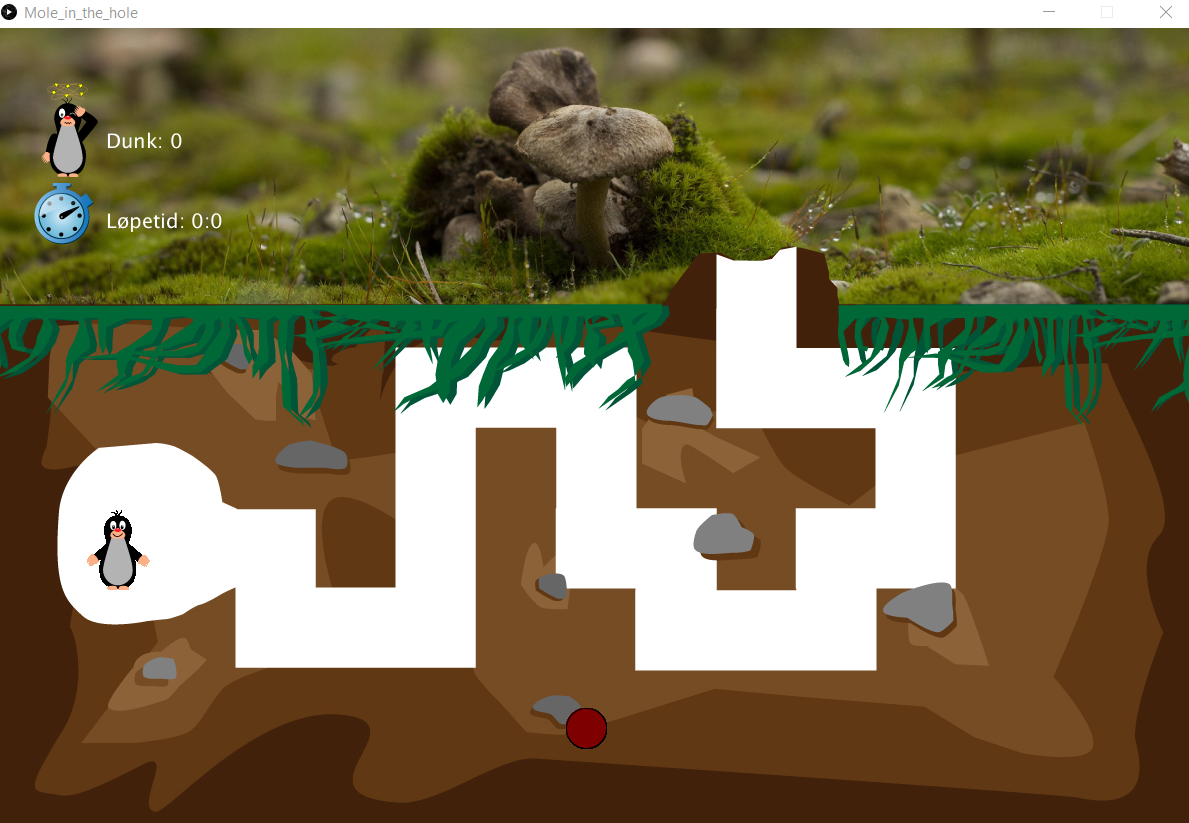
\includegraphics[width=.5\textwidth]{figures/StateStart-Mole_in_the_hole.png}
  \caption[Mole in the hole state start.]{Mole in the hole. State: start.}
  \label{fig:setup}
\end{figure}
\begin{figure}[h]  %t top, b bottom, p page | you can also use h to try to get the figure to appear at the current location
  \centering
  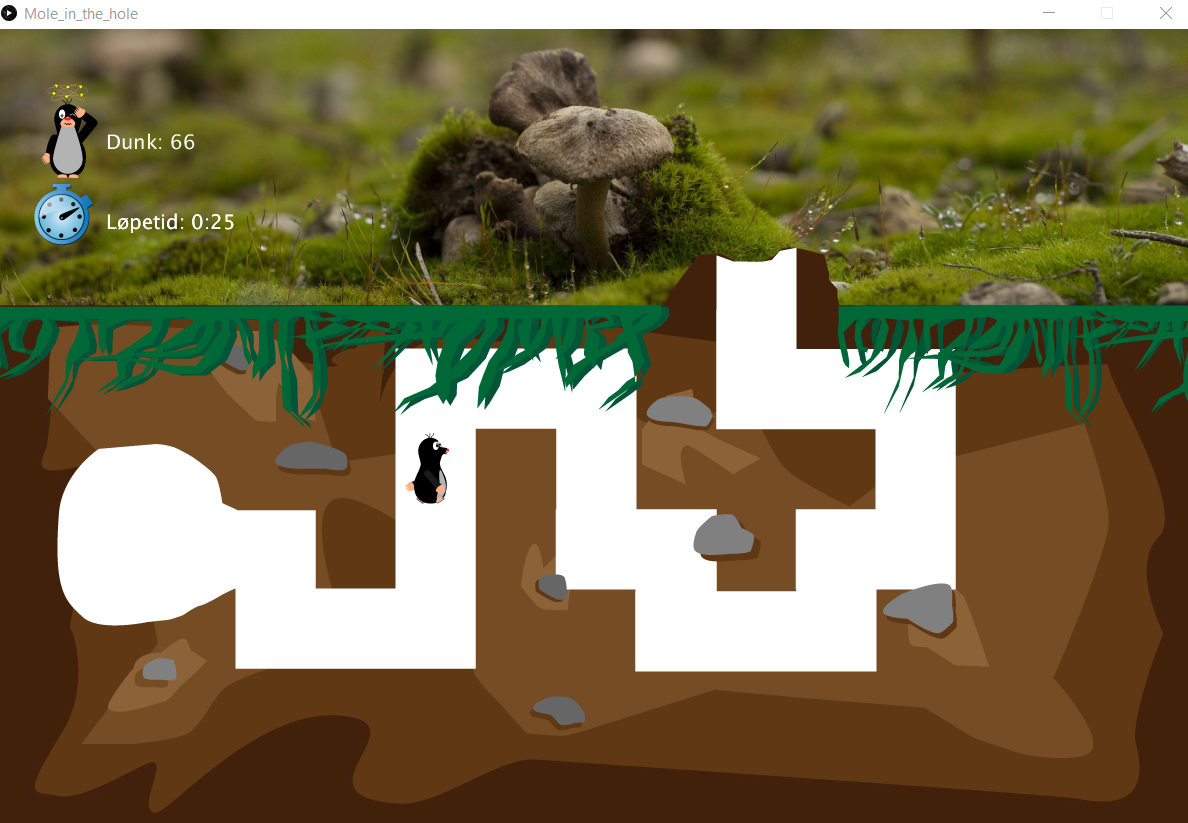
\includegraphics[width=.5\textwidth]{figures/StateGo-Mole_in_the_hole.png}
  \caption[Mole in the hole state go.]{Mole in the hole. State: go.}
  \label{fig:setup}
\end{figure}
\begin{figure}[h]  %t top, b bottom, p page | you can also use h to try to get the figure to appear at the current location
  \centering
  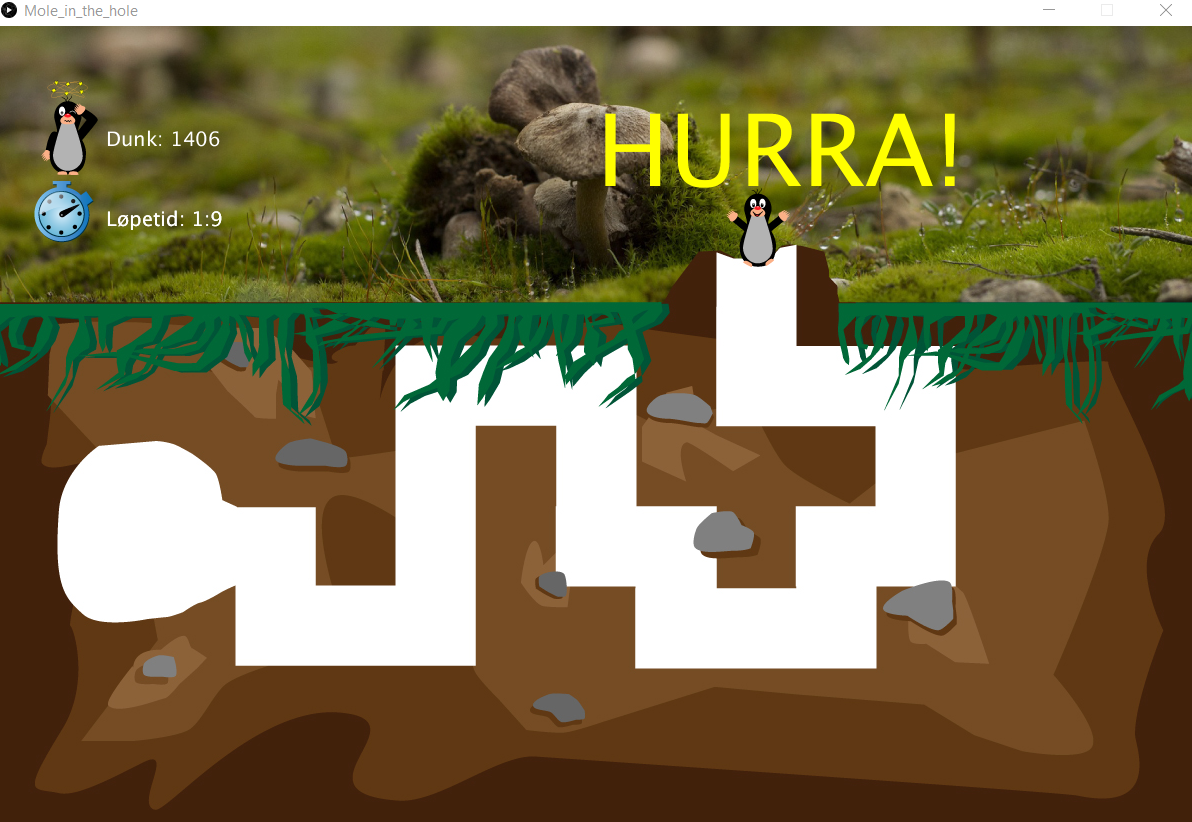
\includegraphics[width=.5\textwidth]{figures/EndState_Mole_in_the_hole.png}
  \caption[Mole in the hole state end.]{Mole in the hole. State: end.}
  \label{fig:setup}
\end{figure}



\subsection{Limitation}
time limit
money? budget
poor code quality
equipment limitation

\section{Experiment }
\label{sec:experiment}


\subsection{Participant}
\label{sec:participant}

The success of this project did not only dependent on the equipment and software but also on voluntaries. Luckily,  parents that saw the value of this research wanted to contribute. A social network as recruiting source was substantial in this situation. The target group for this study ranged from 2 - 13 and should be a good mixture of females and males.
The motive behind the young target group is mainly to check how you a child can be to understand the idea of manipulating a system touch-less and with different gesture. 

According to www.usertest.com, it is recommend to divide children into specific age groups. The main reason for that is the remarkable differences in development of cognitive, physical and social skills. For instance, fine-motor skill are less developed in a 3 year old child than i an a 10 year old.

All in all, 10 young participants, (boys and girls) were recruited for this usability study.


\subsection{Test environment and implementation strategy}
\label{sec:environmnent}

The project is about gaining meaningful data from a gesture-based application when screening children for fine motor deficiency
Working with children can be fun but also challenging at the same time. It needs a certain sensitivity and understanding of children's behaviour and feelings. Children can feel insecure  and anxious in a new environment which could make testing more stressful which probably would result in a wrong outcome. For that reason, each test was conducted at the child's home - a familiar and save environment. Since the equipment was portable, changing the test environment for each participant was not a concern.
Furthermore, in order to gain meaningful data from the experiment, a child's cooperation was necessary.  After a long day at daycare or at school, kids are usually tired and unfocused and hard to motivate. That is especially the case of younger children. For that reason, the experiments were carried out during the weekend and public holidays.  

The time duration needed to complete the task was estimated to 15 minutes. That included 3 attempts and answering the follow up questions. Additionally, extra 20 - 30 minutes were planned for presentation, introduction, equipment setup, debriefing and final thank-you-conversation.

\subsection{Compensation}

According to Nielsen [1998], compensating test users is common. The value of the compensation depends on the type of study and participants. However, he suggested a nice toy or 10 - 15\$ for children or students.
In this study, every child got a small compensation for their contribution. A collection of toys, games, book and other things were offered to choose from. This showed to be a good motivational tool and the children were eagerly to participate and accomplished the task.  

https://www.nngroup.com/articles/when-to-outsource-recruiting-test-users/



\subsection{Equipment}

The equipment for the experiment consisted of a laptop, an external screen and a gesture sensor (Leap Motion). 

\begin{figure}[h]  %t top, b bottom, p page | you can also use h to try to get the figure to appear at the current location
  \centering
  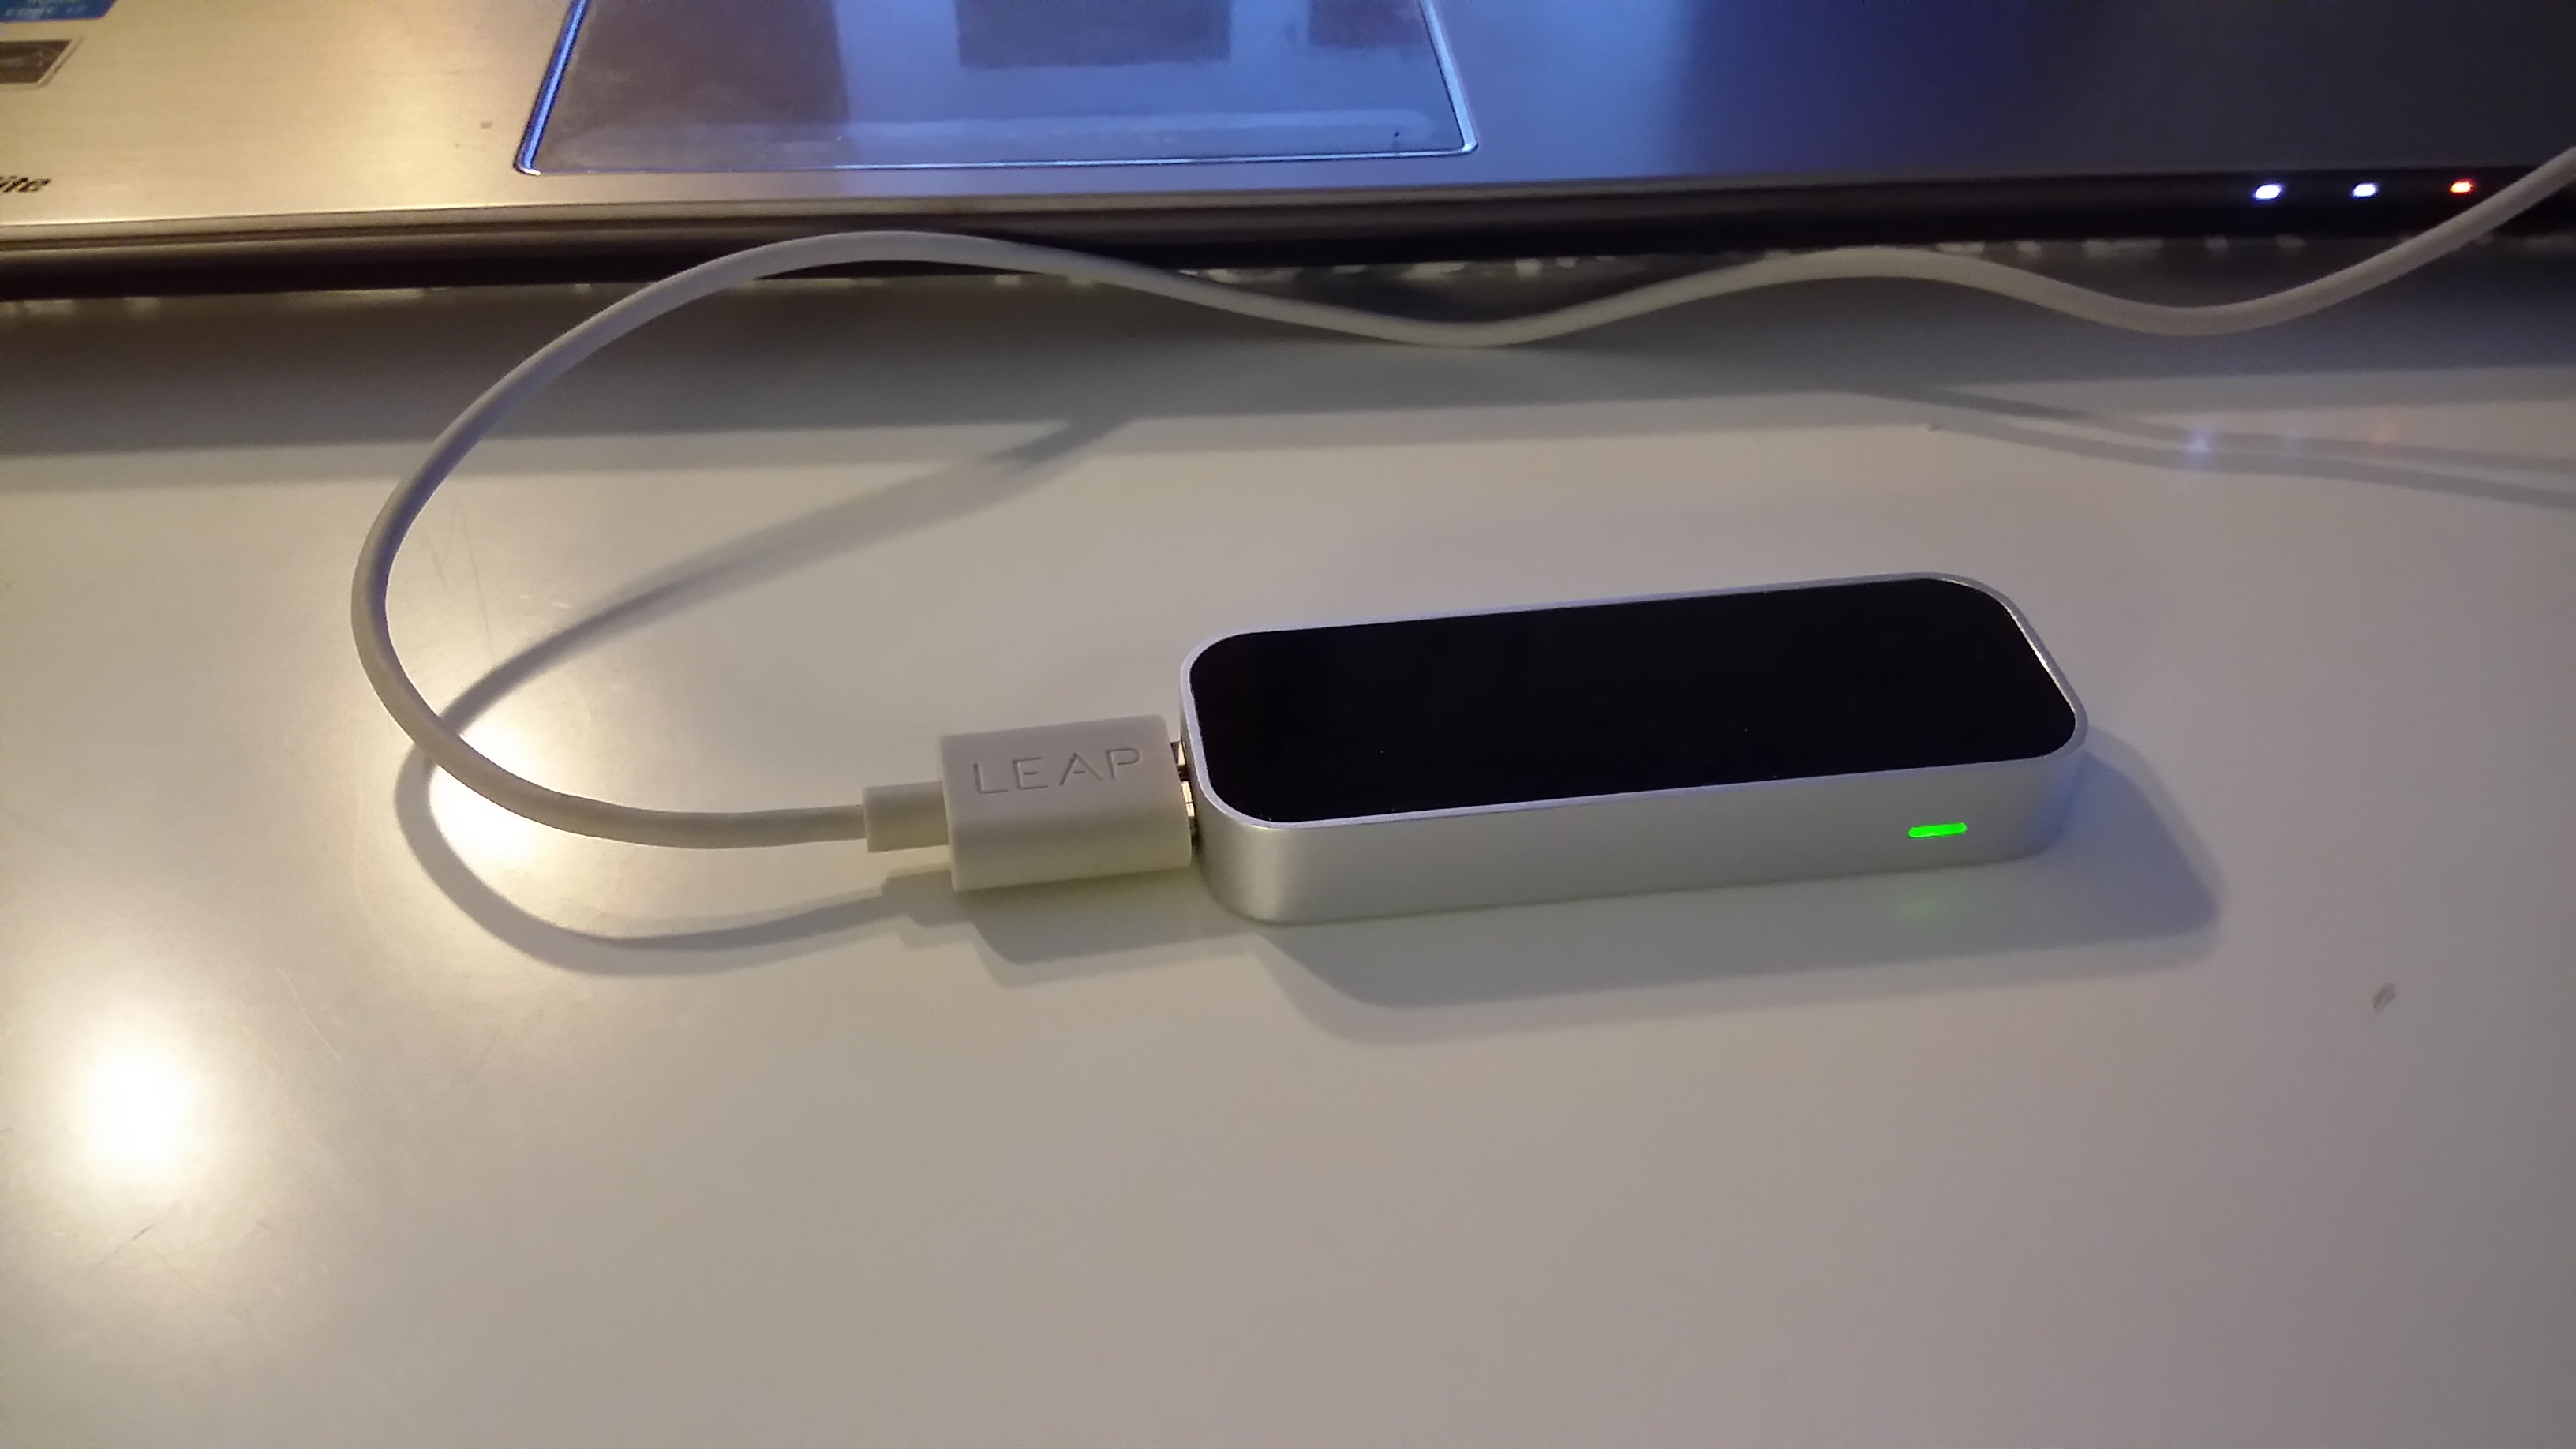
\includegraphics[width=.5\textwidth]{figures/LMdevice.jpg}
  \caption[Leap Motion device.]{Leap Motion device.}
  \label{fig:setup}
\end{figure}

The set up of the equipment needed to be straight forward and fast. An external screen and the Leap Motion device were placed on the table in front of the child. Both, screen and scanner were connected to the laptop. The laptop was place in a way so that the laptop’s screen was not in vision of the test person. All sound that could disturbed during the test session was turned off and the test person could so focus completely on the task.

\begin{figure}[h]  %t top, b bottom, p page | you can also use h to try to get the figure to appear at the current location
  \centering
  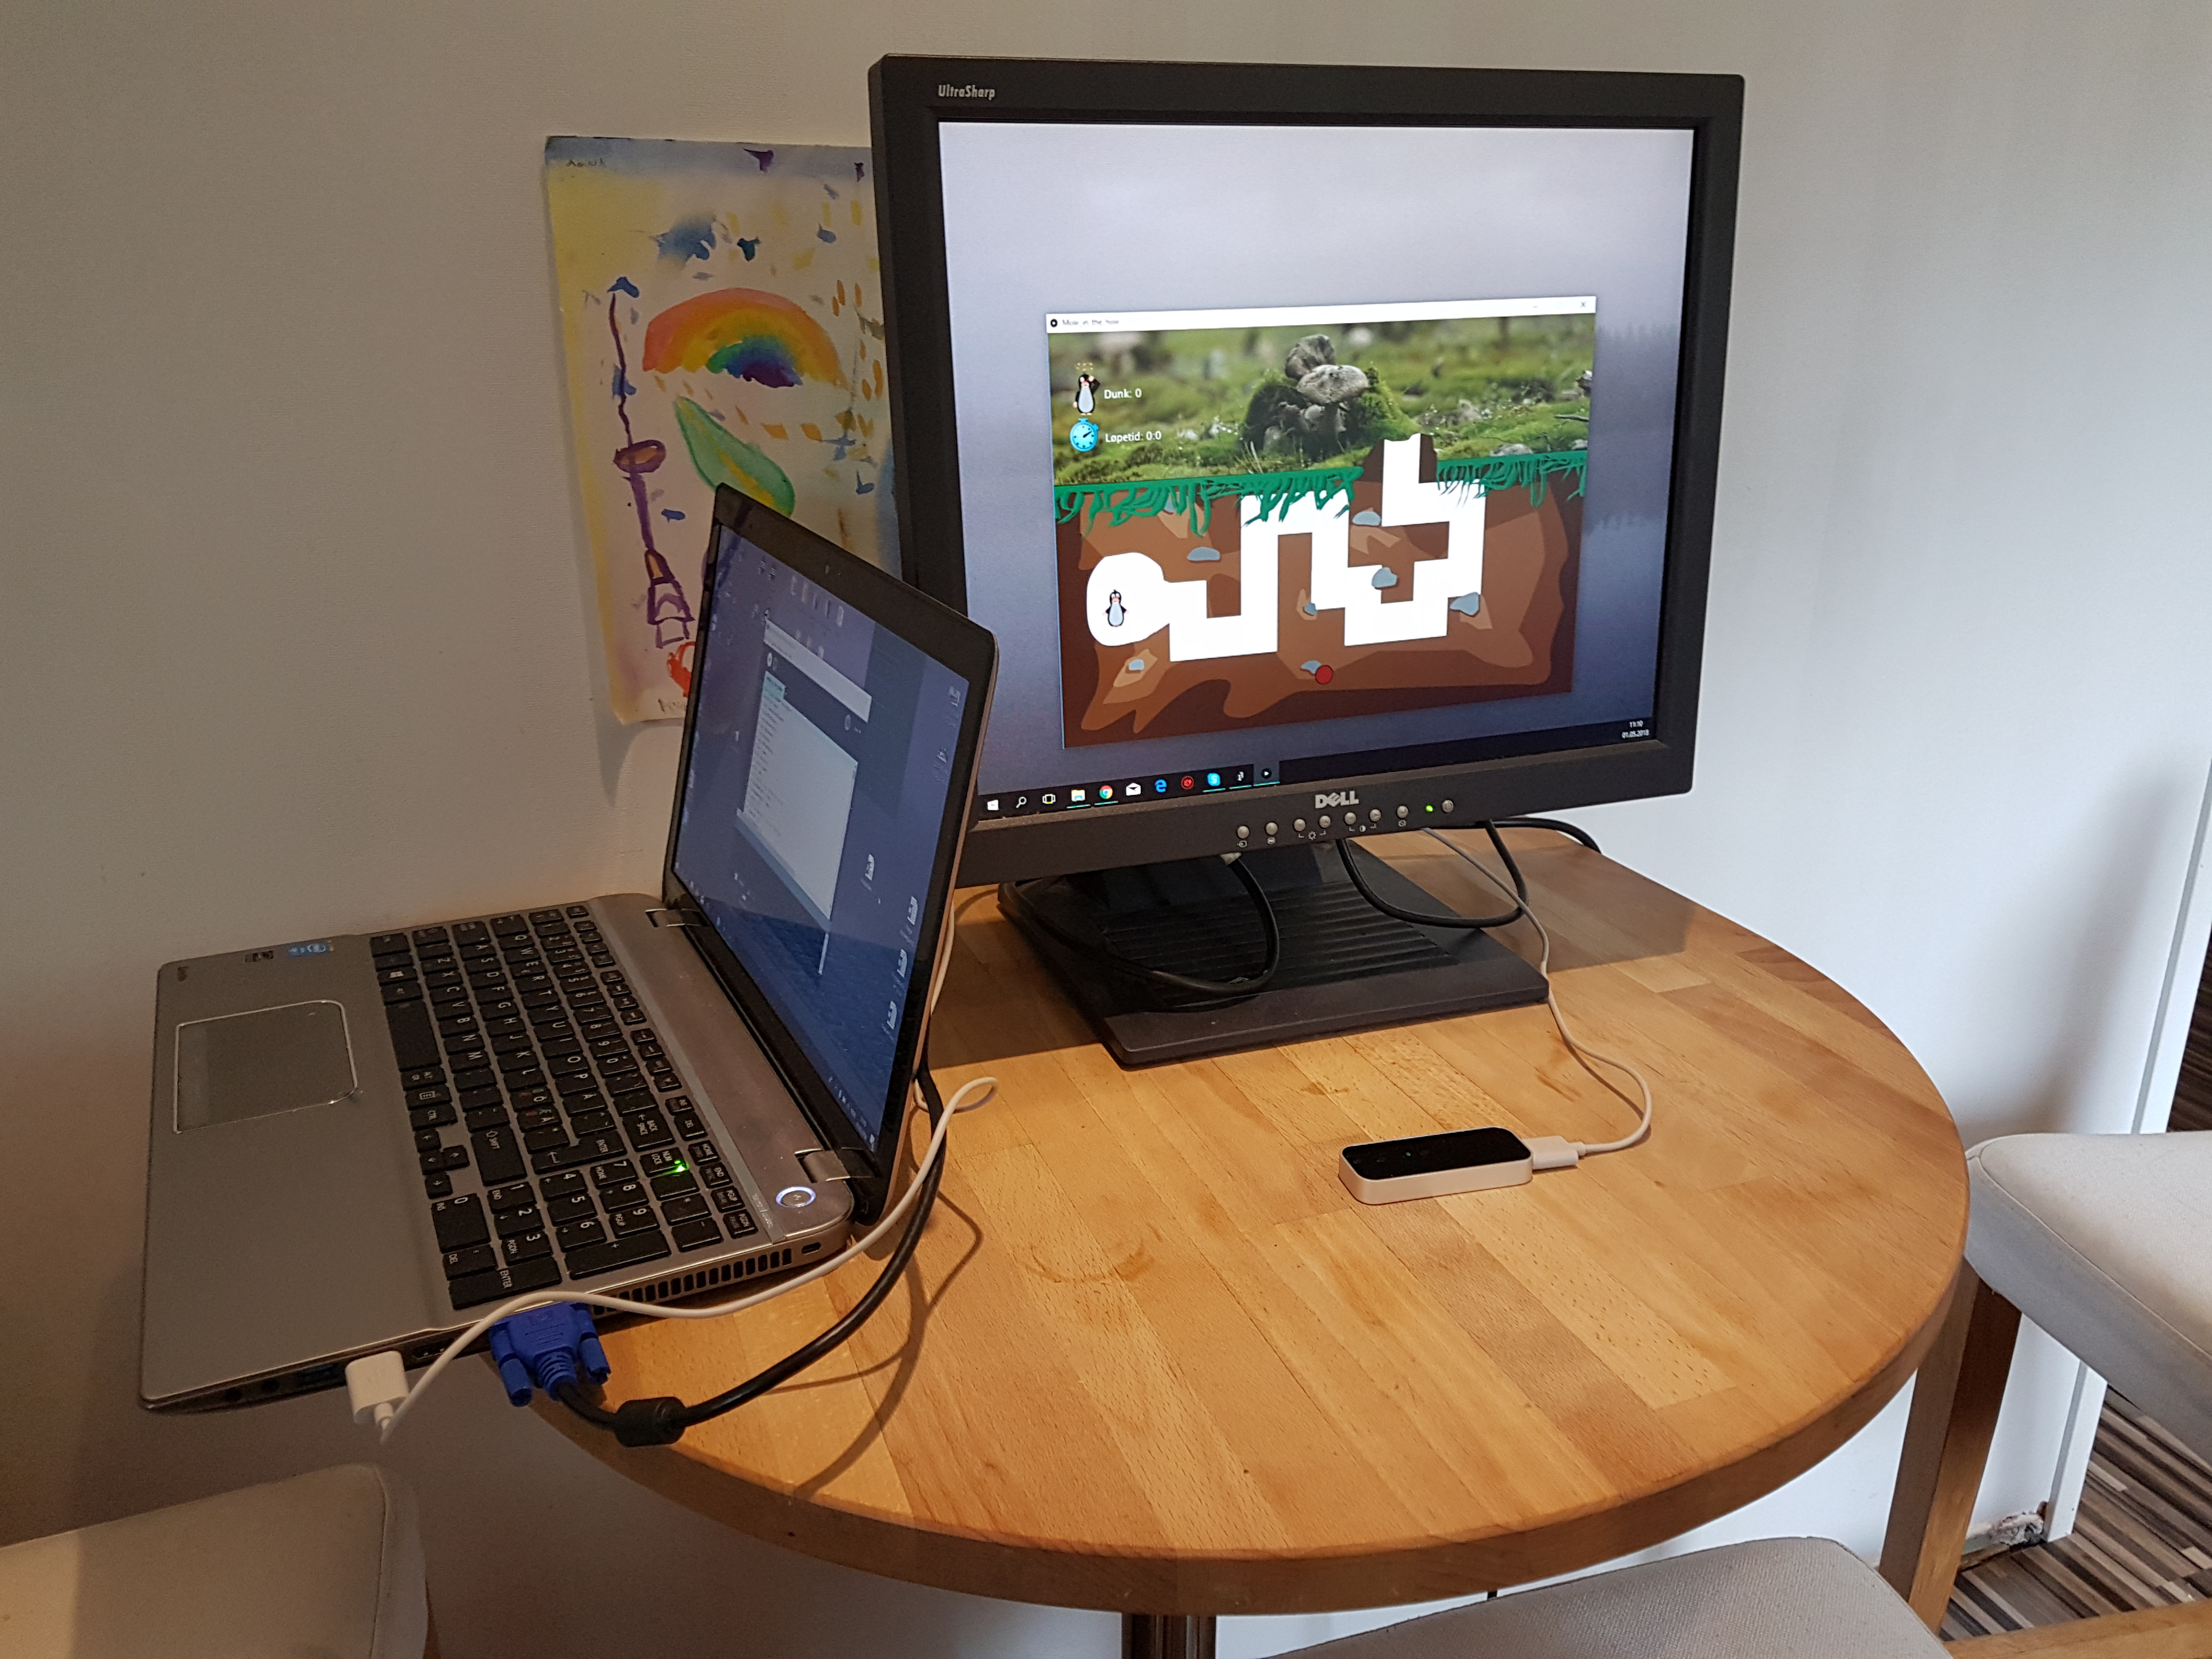
\includegraphics[width=.5\textwidth]{figures/setup.jpg}
  \caption[Equipment setup.]{Equipment setup.}
  \label{fig:setup}
\end{figure}


\subsection{Ethical consideration}
\label{sec:ethical}

Studies involving human participants require considerations of ethical aspects. Children in particularly have to be protected from doubtful research. In this study, ethics, confidentiality and privacy was an important factor during the whole project.
During the experiment, the children were never forced to carry out the task. All involvement was based on voluntary participation. If for any reason a child wasn't cooperative the experiences was canceled immediately. 
It is important to point out that the study didn't collect any personal data. Every participant was registered with a consecutive number which would not reveal the participant identity. The collected data was kept confidential. Only the overall outcome was used for further analysis in order to confirm the hypothesis.  

A concern form was handed to the parents to confirm and sign. The form was downloaded from www.usability.gov and modified for this study. (see attached concern form)


\subsection{Pilot test}

A pilot test was conducted before the real test in order to fine-tune the prototype and test routine and to check if there a other issues to be considered. 
https://www.nngroup.com/articles/pilot-testing/

The person recruited for the pilot test was a young girl in her early teens. She had no pre-experience in hands free gesture applications and was therefore suitable for the task.
The pilot test was conducted some days before the real test.

\begin{figure}[h]  %t top, b bottom, p page | you can also use h to try to get the figure to appear at the current location
  \centering
  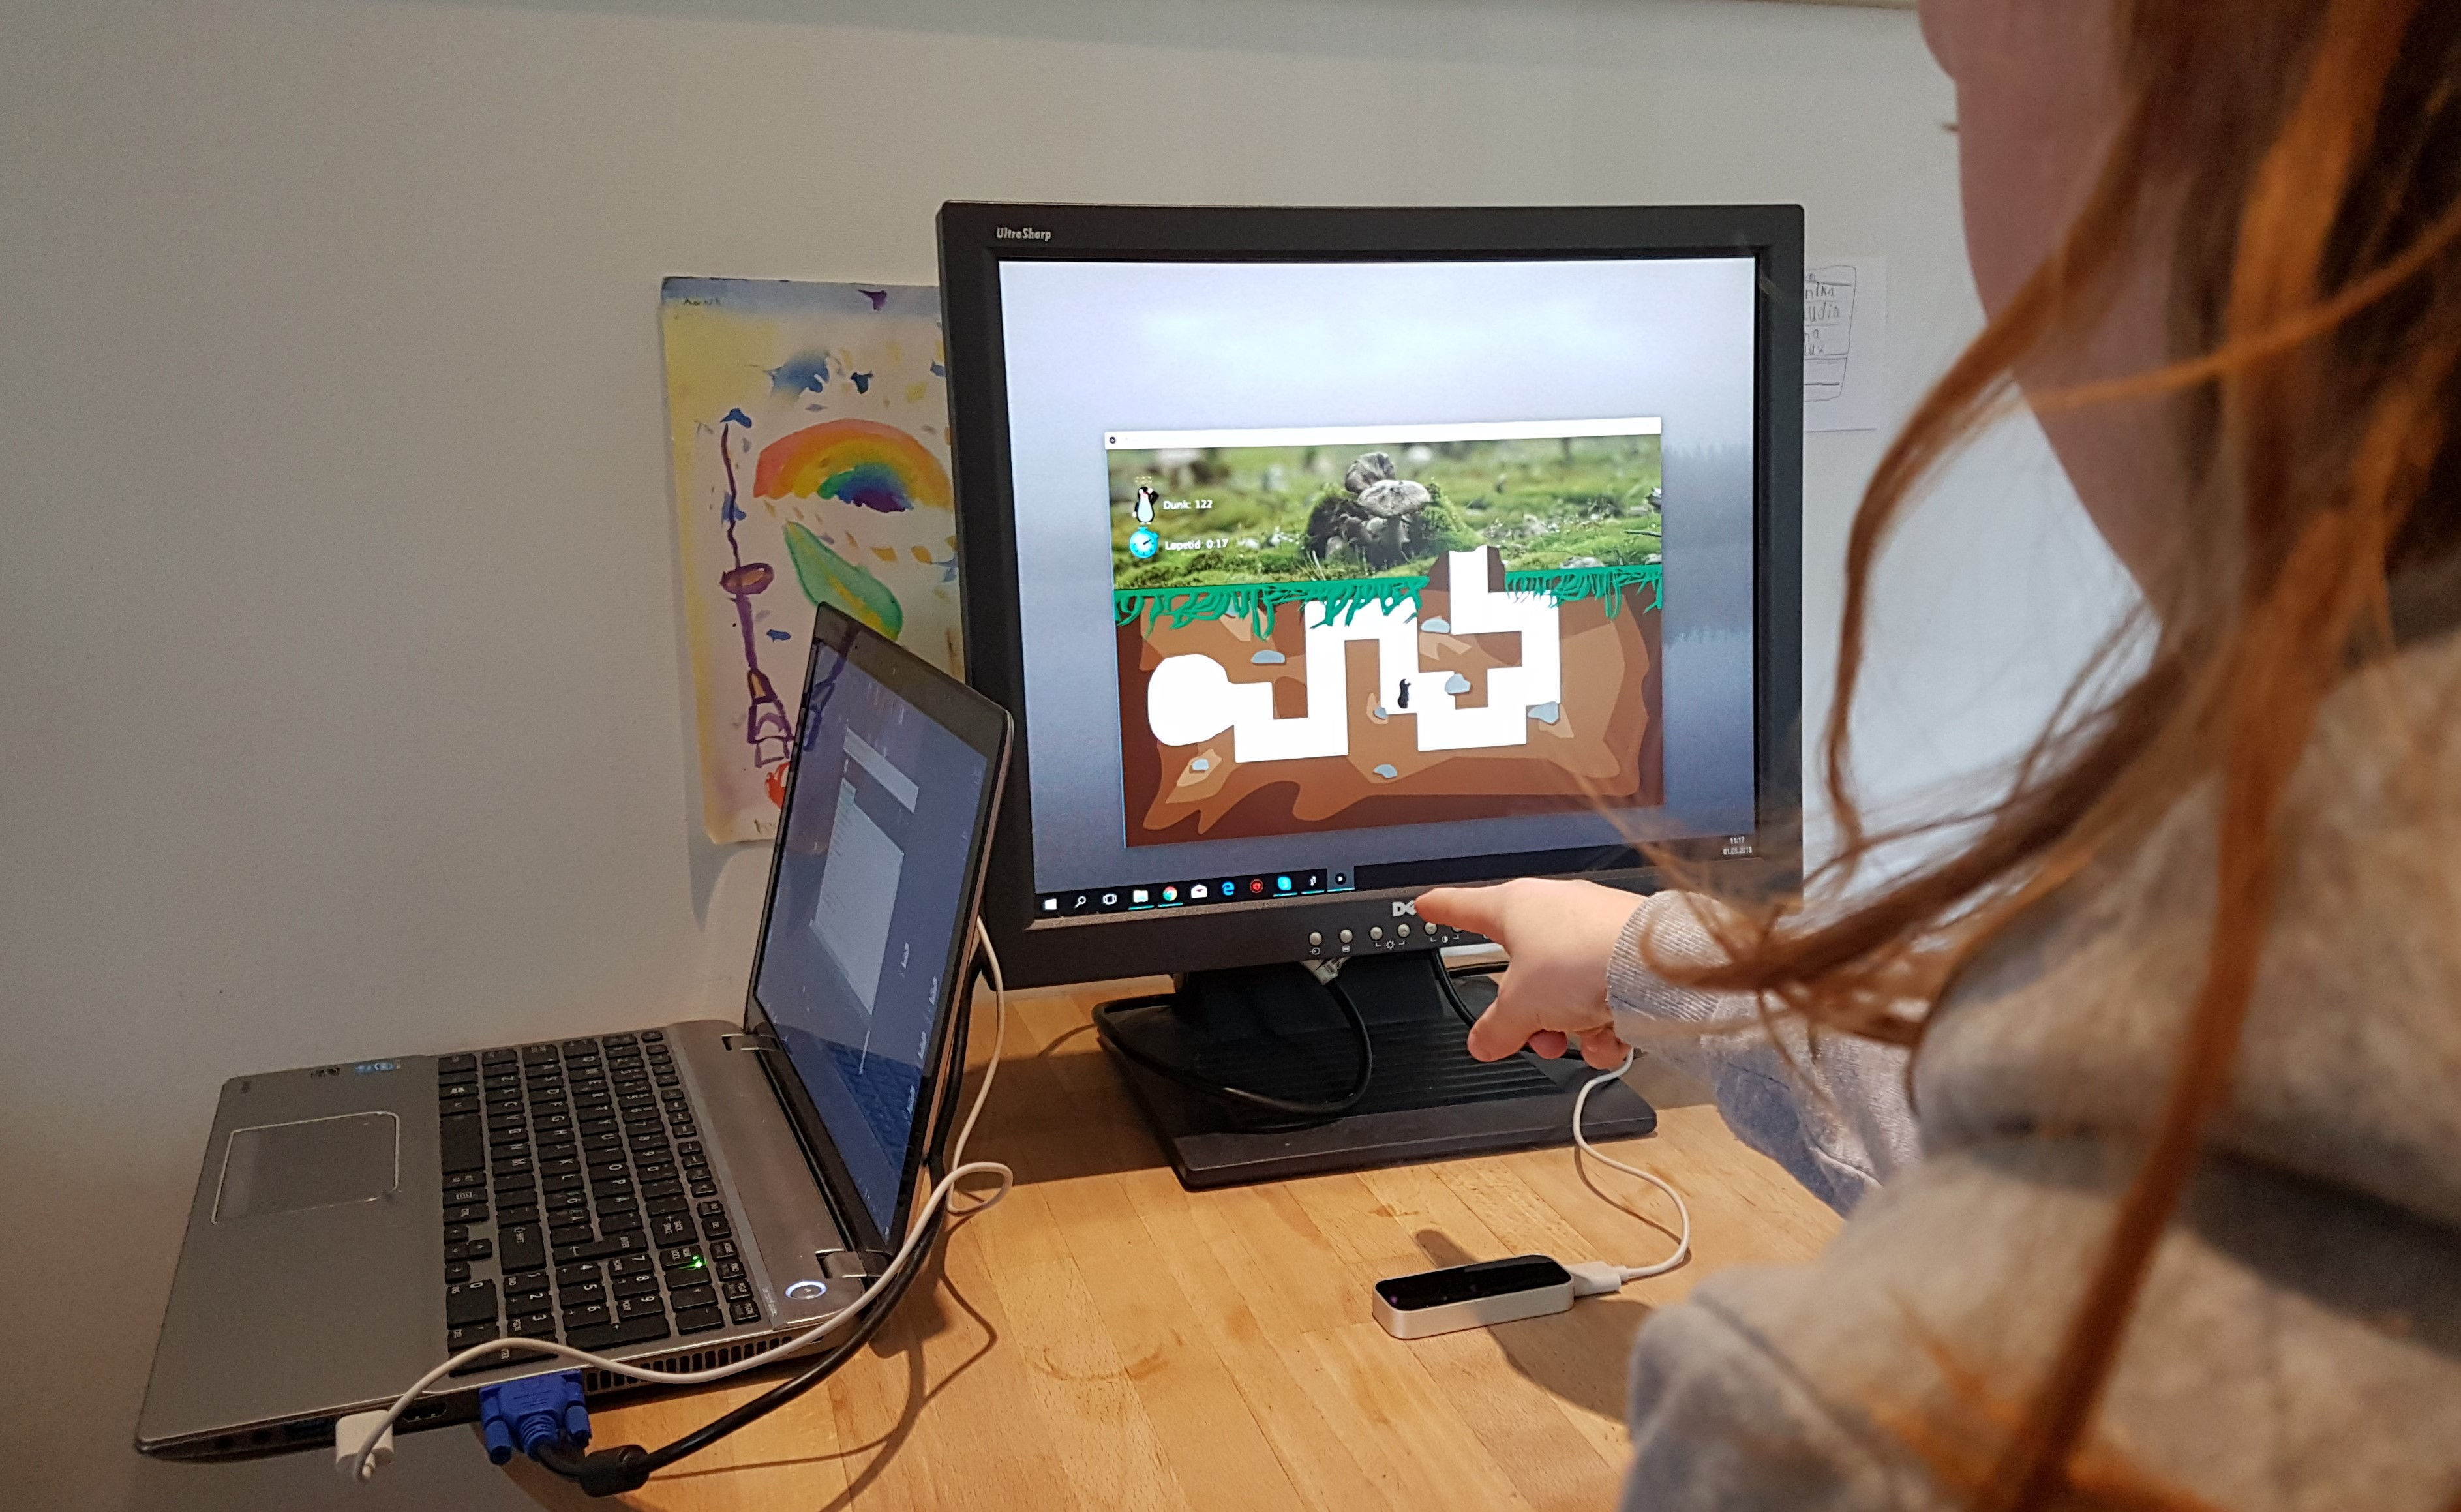
\includegraphics[width=.5\textwidth]{figures/pilottest.jpg}
  \caption[Pilot test.]{Pilot test.}
  \label{fig:setup}
\end{figure}

The pilot test revealed some few issues that needed to be improved or at least to be considered in the real test.  One of the issues concerned the understanding of the system. Since the freehand sensor is a device that still is quite unknown to children,  it is  not enough to say what the participant has to do, but it is  essential to show in advanced how the application works.

The second issue that needed to pay attention is the smiley scale. Since there are different smiley for the scales. Hard-easy and good - bad. It was not a good idea to have them all laid out in front of the participant since this leads to confusion.

The test showed that is was a good idea to have an external screen that only showed the application. 

Furthermore, the test reveal that it is an advantage if the table and the chair have a proper proportion and stands  in relation to the child's body high.

 
The pilot test confirmed the estimated time of 15 minutes of a test run. Additionally 15 min to build up the equipment, have a little conversation with the child, and debriefing.

\subsection{Task description and execution of the usability study}

The purpose behind the usability study was to investigate if the children understand the idea of hand-free interaction. Additionally, the extracted parameters served further analysis. The idea behind that, was to consider a hand-free interaction for medical examination and diagnostic tool. The task of the usability study was about moving the pointer to the mole and than move the mole to the exit as fast as possible while staying on the white path.
The kids also had to perform two gestures in additional, a pointer gesture and a poke gesture. The pointer gesture was needed to navigate and control the game and the poke gesture activated the mole-go-state.

The usability study was planned in advanced on weekends and holidays. Families are usually quite busy and it was quit convenient to organize a meeting on those days.
The equipment was carried and build up at every location on a dinner or kitchen table.

The young participant got explained what kind of technology is used in this usability study, how the Leap motion device works and what the task is.

Considering the still unknown technology, the test moderator showed the participant what the game is about and how to play it. 




\section{Questionnaires}

A short questionnaire was created and used as follow up questions. The questions were about child's own opinion on difficulty, fun, understanding of the game. For the younger participants a smiley scale was create to make the answers more visual and fun and to see if they understand the different facial expression.
The visual scale range from  good - ok to not good and from easy - ok to hard.

\begin{figure}[h]  %t top, b bottom, p page | you can also use h to try to get the figure to appear at the current location
  \centering
  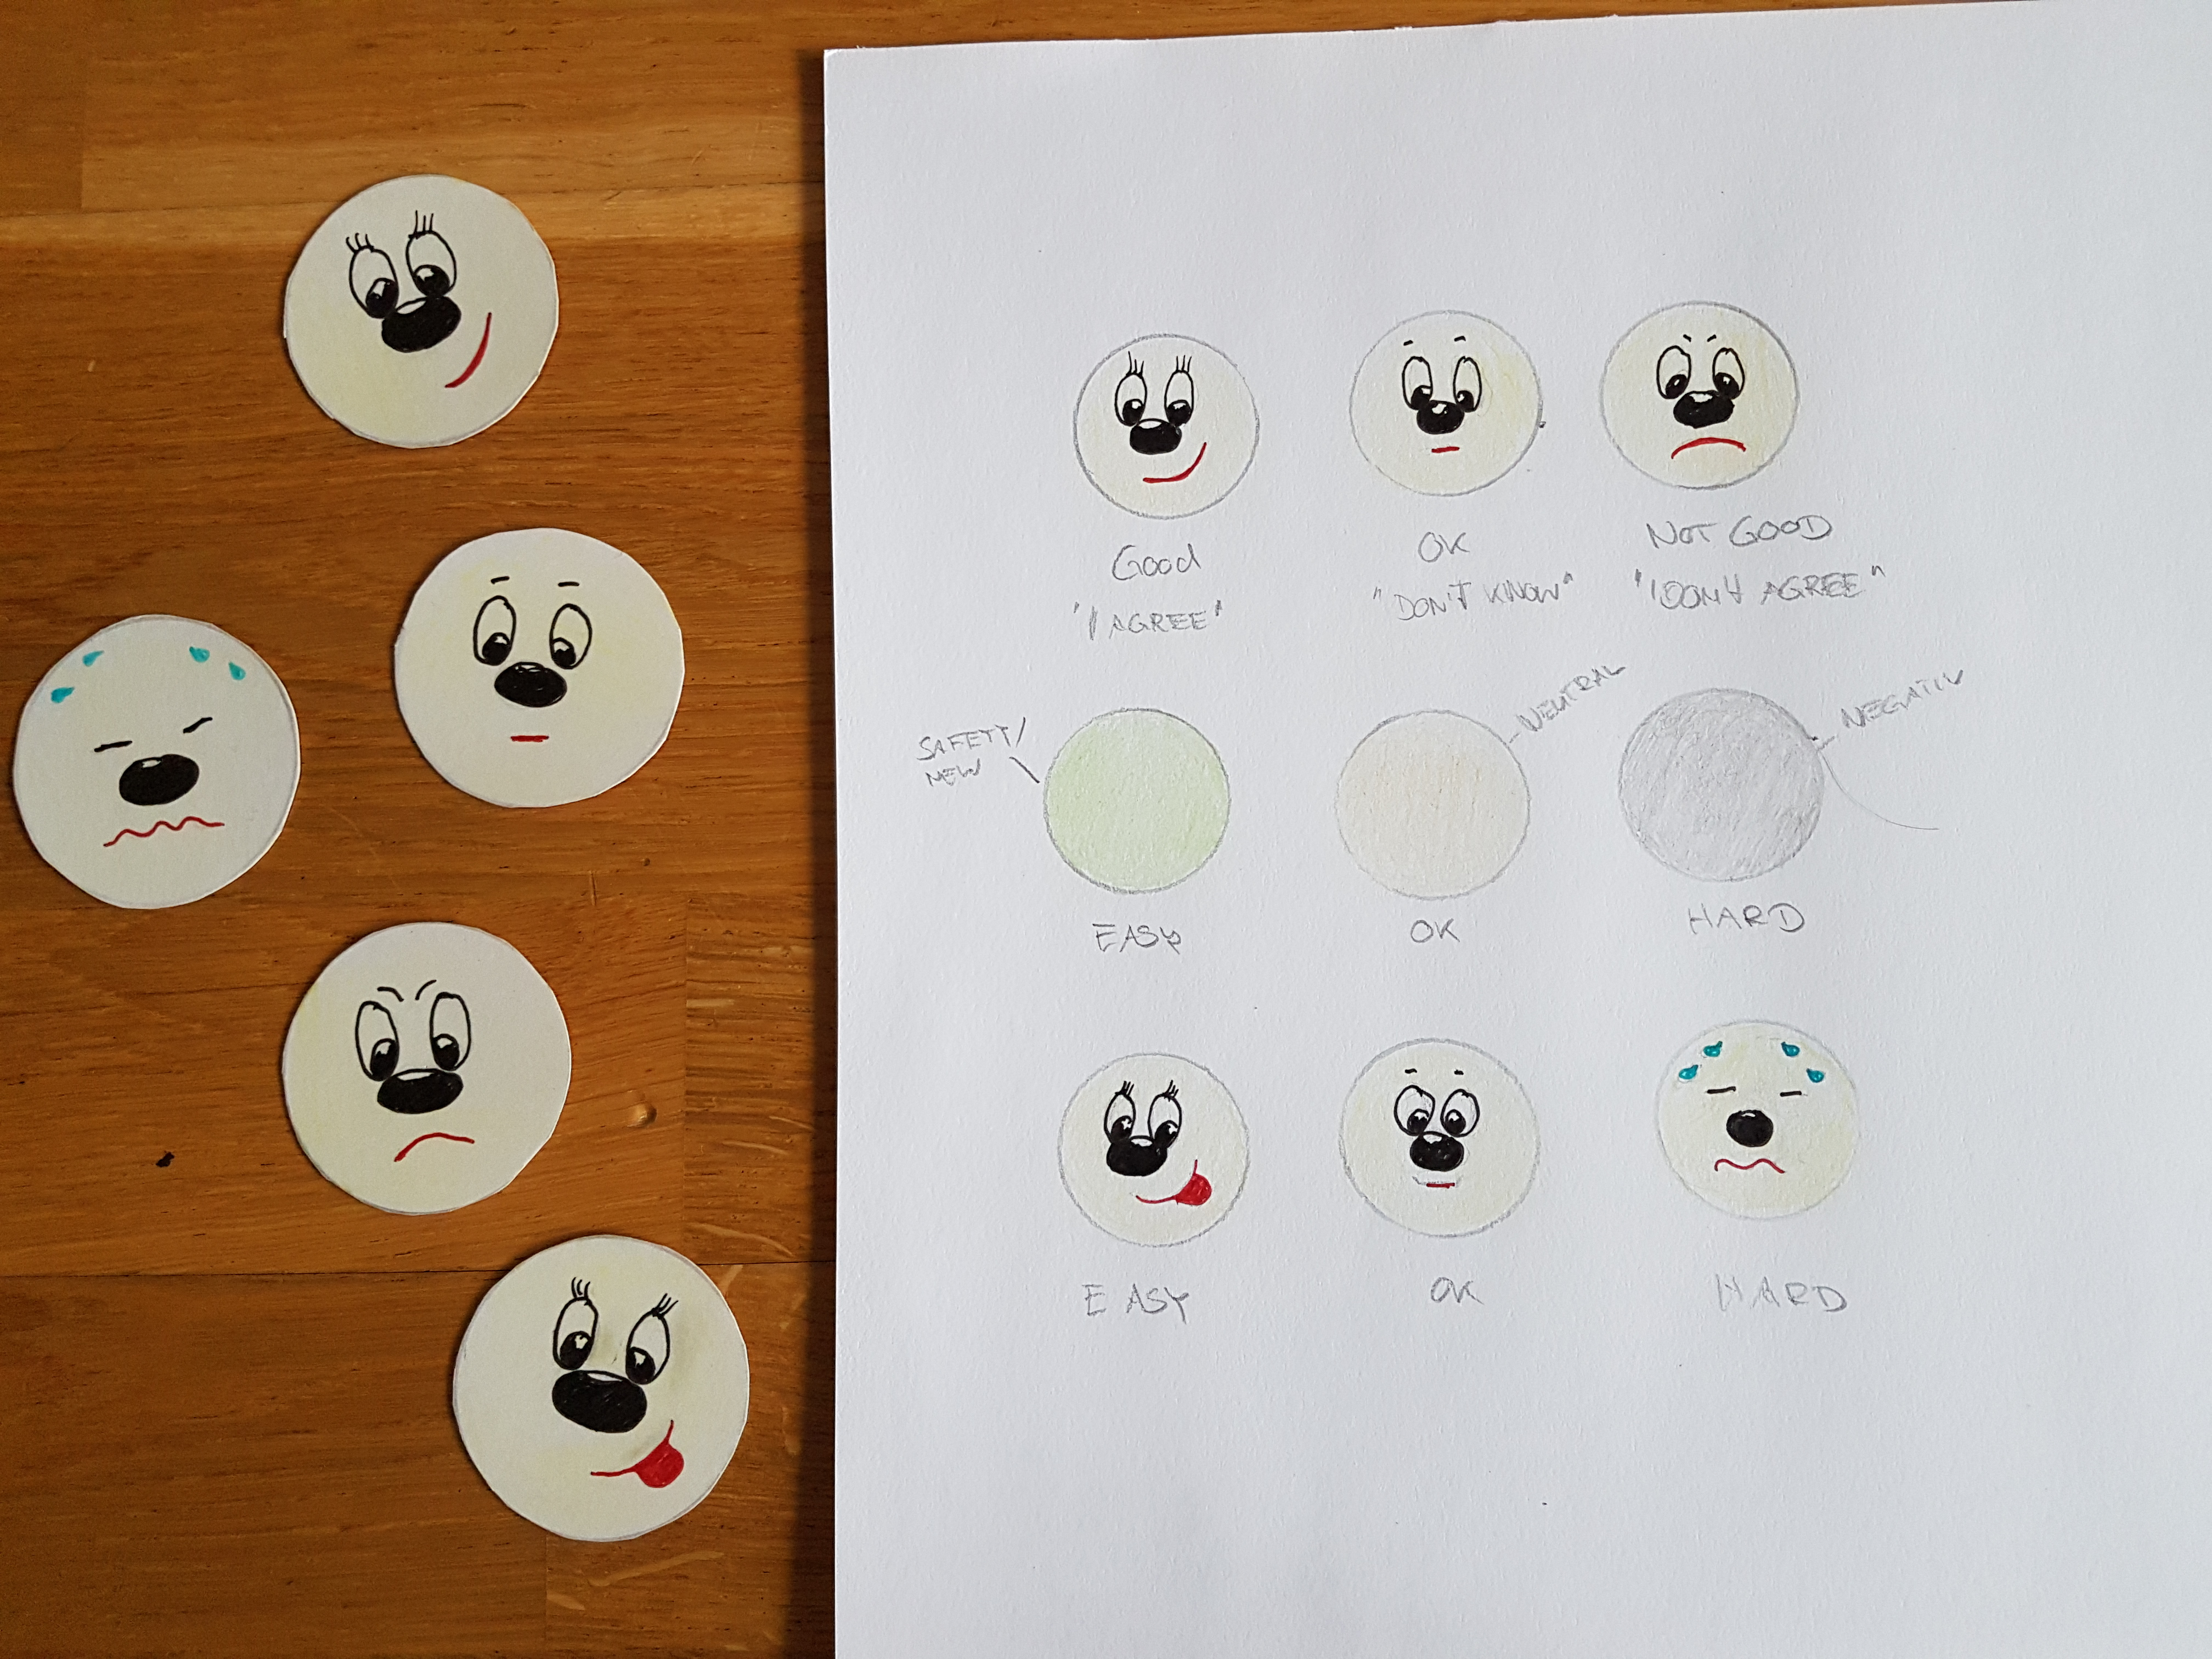
\includegraphics[width=.5\textwidth]{figures/scale.jpg}
  \caption[Visual scale.]{Visual scale.}
  \label{fig:setup}
\end{figure}

The gathered information and data is evaluated and presented in chapter~\ref{chap:dataanalysis} and will be further discussed in chapter~\ref{chap:discussion}.

(see attached questionnaire in the the attachment section.)



\section{Observations}

Observation is a common scientific method and often used in research projects.[reference] 
Observation during this experiment focused on the child's behaviour and reaction during the experiment. Additionally,the ability to perform the task and how much assistance was needed was recorded.